\section{Clase 15}
\subsection{Teoría de campos relativista clásicos}
De la mecánica clásica sabemos que la densidad Lagrangeana debe depender de los campos y de sus primeras derivadas, además de las coordenadas. Esto con el objeto de tener ecuaciones de movimiento de segundo orden en los campos. 

La densidad de Lagrange $\mathcal{L}=\mathcal{L}(\psi,\partial\psi,x)$. El principio de Hamilton nos permite obtener las ecuaciones de movimiento (también llamadas ecuaciones de campo. 

El Lagrangeano es dado por $L=\int\dd^3x \mathcal{L}(\psi,\partial\psi,x)$.

 La acción es dada por
\begin{equation}
  S=\int L\dd t=\int_\Omega\dd^4x \mathcal{L}(\psi,\partial\psi,x)
\end{equation}

\subsubsection{Variación $\db$}
Consideremos variaciones que dejan la región de integración $\Omega$ del espacio-tiempo sin cambios. Esta variación se denota con $\db$, \textit{la cual compara dos campos $\psi$ y $\psi'$ en el mismo punto del espacio-tiempo}. Los campos en el borde de la región $\Omega$ no cambian, esto es,
\begin{equation}
  \eval{\db\psi}_{B=\partial\Omega}=0
\end{equation}
\begin{equation}
  \implies \db\psi(x)=\psi'(x)-\psi(x)
\end{equation}
\begin{equation}
  \implies \psi'(x)=\psi(x)+\db\psi(x)
\end{equation}
de manera que las variaciones $\db$ actuan como
\begin{equation}
  \db : \psi(x)\to \psi'(x)
\end{equation}
es decir, sólo cambian los campos. De aquí, es directo que
\begin{equation}
  \db x^\m =x'^\m -x^\m =0,\implies [\db, \partial_\m ]=0
\end{equation}
Así entonces,
\begin{align}
  \db S&=\db \int_\Omega\dd^4x\mathcal{L}(x)=\int_\Omega\db \mathcal{L}(x)
\end{align}
pero,
\begin{align}
  \db \mathcal{L}(x)&=\db \mathcal{L}(\psi,\partial\psi,x)\\
  &=\pdv{\mathcal{L}}{\psi}\db \psi +\pdv{\mathcal{L}}{(\partial_\m \psi)}\db (\partial_\m \psi)+\pdv{\mathcal{L}}{x^\m }\cancelto{0}{\db x^\m }\\
  &=\pdv{\mathcal{L}}{\psi}\db \psi+\partial_\m \left[\pdv{\mathcal{L}}{(\partial_\m \psi)}\db \psi\right]-\partial_\m \left[\pdv{\mathcal{L}}{(\partial_\m \psi)}\right]\db\psi\\
  &=\left[\pdv{\mathcal{L}}{\psi}-\partial_\m \left(\pdv{\mathcal{L}}{(\partial_\m \psi)}\right)\right]\db\psi -\partial_\m \left[\pdv{\mathcal{L}}{(\partial_\m \psi)}\right]\db\psi
\end{align}
lo que implica que
\begin{align}
  \db S&=\int_\Omega\dd^4x \left[\pdv{\mathcal{L}}{\psi}-\partial_\m \left(\pdv{\mathcal{L}}{(\partial_\m \psi)}\right)\right]-\int_\Omega\dd^4x \partial_\m \left(\pdv{\mathcal{L}}{(\partial_\m \psi)}\db \psi \right)\\
  &=\int_\Omega\dd^4x [\mathcal{L}]\db\psi -\int_{\partial\Omega}\dd S_\m \pdv{\mathcal{L}}{(\partial_\m \psi)}\db \psi=0\\
  &=\int_\Omega\dd^4x [\mathcal{L}]\db\psi=0
\end{align}
\begin{equation}
  \implies [\mathcal{L}]=\pdv{\mathcal{L}}{\psi}-\partial_\m \pdv{\mathcal{L}}{(\partial_\m \psi)}=0
\end{equation}

\subsubsection{Variación $\d$}
Ahora consideremos variaciones que cambian la región de integración $\Omega$, denotada por $\d$. Esta variación compara dos campos $\psi$ y $\psi'$ en dos puntos diferentes $x$ y $x'$,
\begin{equation}
  \implies \d x^\m =x'^\m -x^\m \neq 0
\end{equation}
La variación $\d$ se define como
\begin{equation}
  \d\psi=\psi'(x)-\psi(x)
\end{equation}
Es decir, $\d$ cambia $x$ a $x'$ y $\psi$ a $\psi'$. 

\subsubsection{Relación entre $\db$ y $\d$}
\begin{align}
  \db\psi &=\psi'(x)-\psi(x) + \psi'(x')-\psi'(x')\\
  &=\underbrace{(\psi'(x')-\psi(x))}_{\d\psi}-\psi'(x')+\psi'(x)\\
  &=\d\psi - (\psi'(x')-\psi'(x))\label{15.a}
\end{align}
pero
\begin{align}
  \psi'(x')&=\psi'(x+\d x)=\psi'(x)+\d x^\m \partial_\m \psi'(x)+\cdots 
\end{align}
\begin{equation}
  \implies \psi'(x')-\psi'(x)=\d x^\m \partial_\m \psi'(x)
\end{equation}
de \eqref{15.a}
\begin{equation}
  \implies \db\psi =\d\psi -\d x^\m \partial_\m \psi'(x)
\end{equation}
pero $\psi'(x)=\psi(x)-\db\psi(x)$, luego
\begin{align}
  \db \psi&=\d\psi-\d x^\m \partial_\m (\psi(x)+\db\psi(x))\\
  &=\d\psi -\d x^\m \partial_\m \psi(x)-\underbrace{\d x^\m \partial_\m \db \psi(x)}_{\text{segundo orden}}
\end{align}
\begin{equation}
  \implies\boxed{ \db\psi=\d\psi-\partial_\m \psi(x)\d x^\m }
\end{equation}

Hemos dicho que $\partial_\m (\db \psi)=\db(\partial_\m \psi)$, es decir, $[\db,\partial_\m ]\psi=0$. Consideremos ahora
\begin{align}
  \pdv{x^\m}(\d\psi(x))&=\pdv{x^\m }(\psi'(x')-\psi(x))\\
  &=\pdv{\psi'(x')}{x^\m }-\pdv{\psi(x)}{x^\m }+\pdv{\psi'(x')}{x'^\m }-\pdv{\psi'(x')}{x'^\m }\\
  &=\left(\pdv{\psi'(x')}{x'^\m }-\pdv{\psi(x)}{x^\m }\right)+\pdv{\psi'(x')}{x^\m }-\pdv{\psi'(x')}{x'^\m }\\
  &=\d \left(\pdv{\psi(x)}{x^\m }\right)+\pdv{\psi'(x')}{x'^\n }\pdv{x'^\n }{x^\m }-\pdv{\psi'(x')}{x'^\m }\label{15.b}
\end{align}
pero
\begin{align}
  \pdv{x'^\n }{x^\m }&=\pdv{x^\m}(x^\n +\d x^\n )\\
  &=\pdv{x^\n }{x^\m }+\pdv{\d x^\n }{x^\m }\\
  &=\delta^\n_\m +\pdv{\d x^\n }{x^\m }
\end{align}
luego,
\begin{align}
  \pdv{\psi'(x')}{x'^\n }\pdv{x'^\n }{x^\m }-\pdv{\psi'(x')}{x^\m }&=\pdv{\psi'(x')}{x'^\n }\left(\delta^\n_\m +\pdv{\d x^\n }{x^\m }\right)-\pdv{\psi'(x')}{x'^\m }\\
  &=\cancel{\pdv{\psi'(x')}{x'^\m }}+\pdv{\psi'(x')}{x'^\n }\pdv{\d x^\n }{x^\m }-\cancel{\pdv{\psi'(x')}{x'^\m }}\\
  &=\pdv{\psi'(x')}{x'^\n }\pdv{\d x^\n }{x^\m }
\end{align}
Así, de \eqref{15.b}
\begin{align}
  \pdv{x^\m}(\d\psi(x))&=\d \left(\pdv{\psi(x)}{x^\m }\right)+\pdv{\psi'(x')}{x'^\n }\pdv{\d x^\n }{x^\m }
\end{align}
\begin{equation}
  \implies [\partial_\m \d ]\psi\neq 0
\end{equation}

Consideremos de nuevo la acción
\begin{align}
  S&=\int\dd^4x\L 
\end{align}

\begin{figure}[h!]
	\centering
	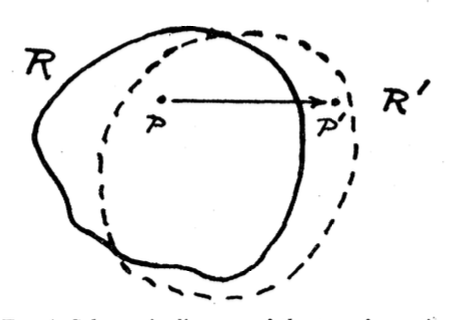
\includegraphics[scale=.5]{fig/img12.png}
\end{figure}
Así,
\begin{align}
  \d S&=\int_{\Omega'}\dd^4x'\L '(x')-\int_\Omega \dd^4x \L (x)\\
\end{align}
donde 
\begin{equation}
  \L(x)=\L (\psi,\partial_\m \psi,x),\qquad \L'(x')=\L' (\psi',\partial'_\m \psi',x')
\end{equation}
y 
\begin{align}
  \d\L(x) &=\L'(x')-\L (x)\implies \L'(x')=\L(x)+\d\L (x)
\end{align}
de manera que
\begin{align}
  \d S&=\int_{\Omega'}\dd^4x'(\L(x)+\d\L (x))-\int_\Omega\dd^4x\L(x)\\
\end{align}
Sabemos que $\dd^4x'$ y $\dd^4x$ se relacionan por $\det$ del Jacobiano,
\begin{align}
  \dd^4x'=J\dd^4x, \qquad \text{con } J=\left|\pdv{x'^\m }{x^\m } \right|
\end{align}
\begin{align}
  J=\left|\pdv{(x^\m +\d x^\m ) }{x^\m } \right|=\left|\pdv{x^\m }{x^\m }+\pdv{\d x^\m }{x^\m }\right|=\left(1+\pdv{\d x^\m }{x^\m }\right)
\end{align}
así,
\begin{align}
  \d S&=\int_{\Omega}\dd^4x\left(1+\pdv{\d x^\m }{x^\m }\right)(\L(x)+\d\L (x))-\int_\Omega\dd^4x\L(x)\\
  &=\int_\Omega\dd^4x \left[\L(x)+\d \L(x)+\pdv{\d x^\m }{x^\m }\L (x)\right]-\int_\Omega\dd^4x\L (x)\\
  &=\int_\Omega\dd^4x\left[\d\L(x)+\pdv{\d x^\m }{x^\m }\L(x)\right]
\end{align}
pero
\begin{equation}
  \d\L(x)=\db\L(x)+\partial_\m \L\d x^\m 
\end{equation}
así
\begin{align}
  \d S&=\int_\Omega\dd^4x\left[\db\L(x)+\partial_\m \L\d x^\m +\partial_\m \d x^\m \L(x)\right]\\
  &=\int_\Omega\dd^4x \left[\db \L(x)+\partial_\m (\L \d x^\m )\right]
\end{align}
pero
\begin{align}
  \db \L(x)=[\L ]\db\psi +\partial_\m \left(\pdv{\L }{(\partial_\m \psi)}\db \psi\right)
\end{align}
luego
\begin{align}
  \d\L &=\db \L +\partial_\m (\L \d x^\m )\\
  &=[\L ]\db\psi+\partial_\m \left(\pdv{\L }{(\partial_\m \psi)}\db \psi+\L \d x^\m\right)\\
  &=[\L ]\db \psi +\partial_\m J^\m 
\end{align}
donde 
\begin{align}
  J^\m &=\pdv{\L }{(\partial_\m \psi)}\db \psi+\L \d x^\m\\
  &=\pdv{\L }{(\partial_\m \psi)}\left(\d \psi-\partial_\n \psi\d x^\n \right)+\L \d x^\m \\
  &=\pdv{\L }{(\partial_\m \psi)}\d\psi -\pdv{\L }{(\partial_\m \psi)}\partial_\n \psi\d x^\n +\L \d x^\m \\
  &=\pdv{\L }{(\partial_\m \psi)}\d\psi +\left(\delta^\m_\n \L -\pdv{\L }{(\partial_\m \psi)}\partial_\n \psi\right)\d x^\n 
\end{align}
Se define,
\begin{align}
  \p^\m &=\pdv{\L }{(\partial_\m \psi)}\\
  T^\m _{~\n }&=\pdv{\L }{(\partial_\m \psi)}\partial_\n \psi-\delta^\m_\n \L 
\end{align}
de manera que
\begin{equation}
 \boxed{ J^\m =\p^\m \delta\psi- T^\m _{~\n }\delta x^\n }
\end{equation}

\subsection{Teoría Electromagnética de Maxwell}
Las ecuaciones de Maxwell vienen dadas por
\begin{align}
  \partial_iE_i &=\frac{\rho}{\epsilon}\label{15.1}\\
  \partial_i B_i&=0\label{15.2}\\
  \epsilon_{ijk}\partial_j E_k&=-\pdv{B_i}{t}\label{15.3}\\
  \epsilon_{ijk}\partial_jB_k&=\m_0 J_i+\m_0\epsilon_0 \pdv{E_i}{t}\label{15.4}
\end{align}
De \eqref{15.2} se tiene que
\begin{equation}
  B_i=\epsilon_{ijk}\partial_j A_k
\end{equation}
\begin{equation}
  \implies \epsilon_{ijk}\partial_j E_k=-\pdv{t}(\epsilon_{ijk}\partial_j A_k)
\end{equation}
\begin{equation}
  \implies \epsilon_{ijl}\partial_j \left(E_k+\pdv{A_k}{t}\right)=0
\end{equation}
\begin{equation}
  \implies E_k=-\partial_k\f -\pdv{A_k}{t}
\end{equation}
Así, las ecuaciones \eqref{15.2} y \eqref{15.3} definen los potenciales electromagnéticos, 
\begin{align}
  \Aboxed{B_i&=\epsilon_{ijk}\partial_j A_k}\\
 \Aboxed{ E_i&=-\partial_i\f -\pdv{A_i}{t}}
\end{align}
La dinámica de estos potenciales vienen determinadas por \eqref{15.1} y \eqref{15.4}.

De \eqref{15.1}
\begin{align}
  \partial_iE_i&=\frac{\rho}{\epsilon_0}\\
  \partial_i\left(-\partial_i\f -\pdv{A_i}{t}\right)&=\frac{\rho}{\epsilon_0}\\
 \Aboxed{ \partial_i\partial_i\f +\pdv{t}\partial_i A_i&=-\frac{\rho}{\epsilon_0}}\label{15.5}
\end{align}
De \eqref{15.4}
\begin{align}
  \epsilon_{ijk}\partial_j(\epsilon_{klm}\partial_l A_m)&=\m_0J_i+\m_0\epsilon_0\pdv{t}\left(-\partial_i\f -\pdv{A_i}{t}\right)\\
  (\delta_{il}\d_{jm}-\d_{im}\d_{jl})\partial_j\partial_l A_m&=\m_0 J_i-\m_0\epsilon_0 \partial_i\pdv{\f}{t}-\m_0\epsilon_0\pdv[2]{A_i}{t}\\
  \partial_j\partial_iA_j-\partial_j\partial_jA_i&=\m_0 J_i-\m_0\epsilon_0\partial_i\pdv{\f }{t}-\m_0\epsilon_0\pdv[2]{A_i}{t}\\
  \partial_j\partial_j A_i-\m_0\epsilon_0\pdv[2]{A_i}{t}&=-\m_0J_i+\partial_i\partial_jA_i+\m_0\epsilon_0 \partial_i\pdv{\f }{t}\\
\Aboxed{ \partial_j\partial_j A_i-\m_0\epsilon_0\pdv[2]{A_i}{t}&=-\m_0J_i+\partial_i\left(\partial_jA_j+\m_0\epsilon_0\pdv{\f }{t}\right)}
\end{align}
De \eqref{15.5}
\begin{align}
  \partial_i\partial_i\f-\m_0\epsilon_0\pdv[2]{\f }{t} &=-\frac{\rho}{\epsilon_0}-\pdv{t}\partial_i A_i--\m_0\epsilon_0\pdv[2]{\f }{t}\\
 \Aboxed{ \partial_i\partial_i\f -\m_0\epsilon_0\pdv[2]{\f }{t}&=-\frac{\rho}{\epsilon_0}-\pdv{t}\left(\partial_iA_i+\m_0\epsilon_0\pdv{\f }{t}\right)}
\end{align}












































































































